\documentclass{ximera}

\graphicspath{{./}{thePythagoreanTheorem/}{deMoivreSavesTheDay/}{complexNumbersFromDifferentAngles/}}

\usepackage{tikz}
\usepackage{tkz-euclide}
\usetkzobj{all}
\tikzstyle geometryDiagrams=[ultra thick,color=blue!50!black]
\newcommand{\tri}{\triangle}
\renewcommand{\l}{\ell}
\renewcommand{\P}{\mathcal{P}}
\newcommand{\R}{\mathbb{R}}
\newcommand{\Q}{\mathbb{Q}}

\newcommand{\Z}{\mathbb Z}

\renewcommand{\vec}{\mathbf}
\renewcommand{\d}{\,d}



%% Egyptian symbols

\usepackage{multido}
\newcommand{\egmil}[1]{\multido{\i=1+1}{#1}{
\includegraphics[scale=.1]{egyptian/egypt_person.pdf}\hspace{0.5mm}}}
\newcommand{\eghuntho}[1]{\multido{\i=1+1}{#1}{
\includegraphics[scale=.1]{egyptian/egypt_fish.pdf}\hspace{0.5mm}}}
\newcommand{\egtentho}[1]{\multido{\i=1+1}{#1}{
\includegraphics[scale=.1]{egyptian/egypt_finger.pdf}\hspace{0.5mm}}}
\newcommand{\egtho}[1]{\multido{\i=1+1}{#1}{
\includegraphics[scale=.1]{egyptian/egypt_lotus.pdf}\hspace{0.5mm}}}
\newcommand{\eghun}[1]{\multido{\i=1+1}{#1}{
\includegraphics[scale=.1]{egyptian/egypt_scroll.pdf}\hspace{0.5mm}}}
\newcommand{\egten}[1]{\multido{\i=1+1}{#1}{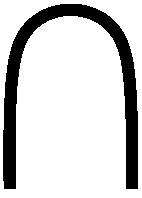
\includegraphics[scale=.1]{egyptian/egypt_heel.pdf}\hspace{0.5mm}}}
\newcommand{\egone}[1]{\multido{\i=1+1}{#1}{
\includegraphics[scale=.1]{egyptian/egypt_stroke.pdf}\hspace{0.5mm}}}
\newcommand{\egyptify}[7]{
 \multido{\i=1+1}{#1}{
\includegraphics[scale=.1]{egyptian/egypt_person.pdf}\hspace{0.5mm}}
 \multido{\i=1+1}{#2}{
\includegraphics[scale=.1]{egyptian/egypt_fish.pdf}\hspace{0.5mm}}
 \multido{\i=1+1}{#3}{
\includegraphics[scale=.1]{egyptian/egypt_finger.pdf}\hspace{0.5mm}}
 \multido{\i=1+1}{#4}{
\includegraphics[scale=.1]{egyptian/egypt_lotus.pdf}\hspace{0.5mm}}
 \multido{\i=1+1}{#5}{
\includegraphics[scale=.1]{egyptian/egypt_scroll.pdf}\hspace{0.5mm}}
 \multido{\i=1+1}{#6}{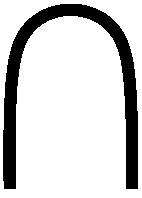
\includegraphics[scale=.1]{egyptian/egypt_heel.pdf}\hspace{0.5mm}}
 \multido{\i=1+1}{#7}{
\includegraphics[scale=.1]{egyptian/egypt_stroke.pdf}\hspace{0.5mm}}
 \hspace{.5mm}
}




\title{The unique factorization theorem}
\begin{document}
\begin{abstract}
In this activity we investigate unique factorization theorems.
\end{abstract}
\maketitle


Consider this proposition from Euclid's \textit{Elements}:

\begin{proposition}[IX.14]
If a number is the least that is measured by prime numbers, then it is
not measured by any other prime number except those originally
measuring it.
\end{proposition}

\begin{question}
Explain what the proposition above is saying.
\end{question}


\begin{question}
Now consider Euclid's proof:
\begin{quote}
Let the number $A$ be the least that is measured by the prime numbers
$B$, $C$, and $D$.  I say that $A$ is not measured by any other prime
number except $B$, $C$, or $D$.  If possible, let it be measured by
the prime number $E$, and let $E$ not be the same as any one of the
numbers $B$, $C$, or $D$.

Now, since $E$ measures $A$, let it measure it according to $F$, therefore $E$
multiplied by $F$ makes $A$. And $A$ is measured by the prime numbers $B$, $C$,
and $D$.  But, if two numbers multiplied by one another make some
number, and any prime number measures the product, then it also
measures one of the original numbers, therefore each of $B$, $C$, and $D$
measures one of the numbers $E$ or $F$.  Now they do not measure $E$, for $E$
is prime and not the same with any one of the numbers $B$, $C$, or
$D$. Therefore they measure $F$, which is less than $A$, which is
impossible, for $A$ is by hypothesis the least number measured by $B$, $C$,
and $D$.  Therefore no prime number measures $A$ except $B$, $C$, and $D$.
Therefore, if a number is the least that is measured by prime numbers,
then it is not measured by any other prime number except those
originally measuring it.
\end{quote}
Can you explain what this proof is saying?
\end{question}

\newpage

Now let's consider a crazy set of numbers---all multiples of
$3$. Let's use the symbol $3\Z$ to denote the set consisting of all
multiples of $3$. As a gesture of friendship, I have written down the
first $100$ nonnegative integers in $3\Z$:


\[
\begin{array}{cccccccccc}
0   & 3   & 6   & 9   & 12  & 15  & 18  & 21  & 24  & 27  \\
\\
30  & 33  & 36  & 39  & 42  & 45  & 48  & 51  & 54  & 57  \\
\\
60  & 63  & 66  & 69  & 72  & 75  & 78  & 81  & 84  & 87  \\
\\
90  & 93  & 96  & 99  & 102 & 105 & 108 & 111 & 114 & 117 \\
\\
120 & 123 & 126 & 129 & 132 & 135 & 138 & 141 & 144 & 147 \\
\\
150 & 153 & 156 & 159 & 162 & 165 & 168 & 171 & 174 & 177 \\
\\
180 & 183 & 186 & 189 & 192 & 195 & 198 & 201 & 204 & 207 \\
\\
210 & 213 & 216 & 219 & 222 & 225 & 228 & 231 & 234 & 237 \\
\\
240 & 243 & 246 & 249 & 252 & 255 & 258 & 261 & 264 & 267 \\
\\
270 & 273 & 276 & 279 & 282 & 285 & 288 & 291 & 294 & 297
\end{array}
\]



\begin{question}
Given any two integers in $3\Z$, will their sum be in $3\Z$? Explain
your reasoning.
\end{question}

\begin{question}
Given any two integers in $3\Z$, will their difference be in $3\Z$?
Explain your reasoning.
\end{question}

\begin{question}
Given any two integers in $3\Z$, will their product be in $3\Z$?
Explain your reasoning.
\end{question}

\begin{question}
Given any two integers in $3\Z$, will their quotient be in $3\Z$?
Explain your reasoning.
\end{question}

\begin{definition}
Call a positive integer \textbf{prome} in $3\Z$ if it cannot be
expressed as the product of two integers \textit{both} in $3\Z$.
\end{definition}

As an example, I tell you that $6$ is prome number in $3\Z$. You may
object because $6 = 2\cdot 3$, but remember---$2$ is not in $3\Z$!


\begin{question}
List all the prome numbers less than $297$.
\end{question}

\begin{question}
Can you give some sort of algebraic characterization of prome numbers
in $3\Z$? 
\end{question}

\begin{question}
Can you find numbers that factor completely into prome numbers in
\textit{two} different ways? How many can you find?
\end{question}

\end{document}
